 \documentclass[answers]{exam}
\newif\ifanswers
\answerstrue % comment out to hide answers

\usepackage{lastpage} % Required to determine the last page for the footer
\usepackage{extramarks} % Required for headers and footers
\usepackage[usenames,dvipsnames]{color} % Required for custom colors
\usepackage{graphicx} % Required to insert images
\usepackage{listings} % Required for insertion of code
\usepackage{courier} % Required for the courier font
\usepackage{lipsum} % Used for inserting dummy 'Lorem ipsum' text into the template
\usepackage{enumerate}
\usepackage{subfigure}
\usepackage{booktabs}
\usepackage{amsmath, amsthm, amssymb}
\usepackage{hyperref}
\usepackage{datetime}
\usepackage{minted}
\settimeformat{ampmtime}
\usepackage{algpseudocode}
\usepackage{algorithmicx}
\usepackage[ruled]{algorithm}
\usepackage{tikz-dependency}
\usepackage{tikz}
\usepackage{changepage}
\usepackage{enumerate}
\usepackage{enumitem}
% \usepackage{bm}
\usetikzlibrary{positioning,patterns,fit,calc}
% Margins
\topmargin=-0.45in
\evensidemargin=0in
\oddsidemargin=0in
\textwidth=6.5in
\textheight=9.0in
\headsep=0.25in

\linespread{1.1} % Line spacing

% Set up the header and footer
%\pagestyle{fancy}
%\rhead{\hmwkAuthorName} % Top left header
%\lhead{\hmwkClass: \hmwkTitle} % Top center head
%\lfoot{\lastxmark} % Bottom left footer
%\cfoot{} % Bottom center footer
%\rfoot{Page\ \thepage\ of\ \protect\pageref{LastPage}} % Bottom right footer
%\renewcommand\headrulewidth{0.4pt} % Size of the header rule
%\renewcommand\footrulewidth{0.4pt} % Size of the footer rule

\pagestyle{headandfoot}
\runningheadrule{}
\firstpageheader{CS 224n}{Assignment 2}{}
\runningheader{CS 224n} {Assignment 2} {Page \thepage\ of \numpages}
\firstpagefooter{}{}{} \runningfooter{}{}{}

\setlength\parindent{0pt} % Removes all indentation from paragraphs

%----------------------------------------------------------------------------------------
%	CODE INCLUSION CONFIGURATION
%----------------------------------------------------------------------------------------

\definecolor{MyDarkGreen}{rgb}{0.0,0.4,0.0} % This is the color used for comments
\definecolor{shadecolor}{gray}{0.9}
\lstloadlanguages{Python} % Load Perl syntax for listings, for a list of other languages supported see: ftp://ftp.tex.ac.uk/tex-archive/macros/latex/contrib/listings/listings.pdf
\lstset{language=Python, % Use Perl in this example
        frame=single, % Single frame around code
        basicstyle=\footnotesize\ttfamily, % Use small true type font
        keywordstyle=[1]\color{Blue}\bf, % Perl functions bold and blue
        keywordstyle=[2]\color{Purple}, % Perl function arguments purple
        keywordstyle=[3]\color{Blue}\underbar, % Custom functions underlined and blue
        identifierstyle=, % Nothing special about identifiers
        commentstyle=\usefont{T1}{pcr}{m}{sl}\color{MyDarkGreen}\small, % Comments small dark green courier font
        stringstyle=\color{Purple}, % Strings are purple
        showstringspaces=false, % Don't put marks in string spaces
        tabsize=5, % 5 spaces per tab
        %
        % Put standard Perl functions not included in the default language here
        morekeywords={rand},
        %
        % Put Perl function parameters here
        morekeywords=[2]{on, off, interp},
        %
        % Put user defined functions here
        morekeywords=[3]{test},
       	%
        morecomment=[l][\color{Blue}]{...}, % Line continuation (...) like blue comment
        numbers=left, % Line numbers on left
        firstnumber=1, % Line numbers start with line 1
        numberstyle=\tiny\color{Blue}, % Line numbers are blue and small
        stepnumber=5 % Line numbers go in steps of 5
}

%----------------------------------------------------------------------------------------
%	NAME AND CLASS SECTION
%----------------------------------------------------------------------------------------

\newcommand{\hmwkTitle}{Word2Vec and Dependency Parsing} % Assignment title
\newcommand{\hmwkClass}{CS\ 224n Assignment \#2} % Course/class
\newcommand{\ifans}[1]{\ifanswers \color{red} \textbf{Solution: } #1 \color{black} \fi}

% \newcommand{\ifans}[1]{}

\input macros.tex
\input std_macros.tex

%----------------------------------------------------------------------------------------
%	TITLE PAGE
%----------------------------------------------------------------------------------------
\qformat{\Large\bfseries\thequestion{}. \thequestiontitle{} (\thepoints{})\hfill}

\title{
\vspace{-1in}
\textmd{\textbf{\hmwkClass:\ \hmwkTitle}}
}
\author{}
%\date{\textit{\small Updated \today\ at \currenttime}} % Insert date here if you want it to appear below your name
\date{}

\setcounter{section}{0} % one-indexing
\begin{document}

\maketitle
\vspace{-3em}

\textbf{Due Date: April 18th, Thursday, 4:30 PM PST.}

In this assignment, you will review the mathematics behind Word2Vec and build a neural dependency parser using PyTorch. For a review of the fundamentals of PyTorch, please check out the PyTorch review session on Canvas. In Part 1, you will explore the partial derivatives involved in training a Word2vec model using the naive softmax loss. In Part 2, you will learn about two general neural network techniques (Adam Optimization and Dropout). In Part 3, you will implement and train a dependency parser using the techniques from Part 2, before analyzing a few erroneous dependency parses.

If you are using LaTeX, you can use \verb!\ifans{}! to type your solutions.

\textbf{Please tag the questions correctly on Gradescope, otherwise the TAs will take points off if you don't tag questions.}
\begin{questions}
    \titledquestion{Understanding word2vec}[15]
Recall that the key insight behind {\tt word2vec} is that \textit{`a word is known by the company it keeps'}. Concretely, consider a `center' word $c$ surrounded before and after by a context of a certain length. We term words in this contextual window `outside words' ($O$). For example, in Figure~\ref{fig:word2vec}, the context window length is 2, the center word $c$ is `banking', and the outside words are `turning', `into', `crises', and `as':

\begin{figure}[h]
    \centering
    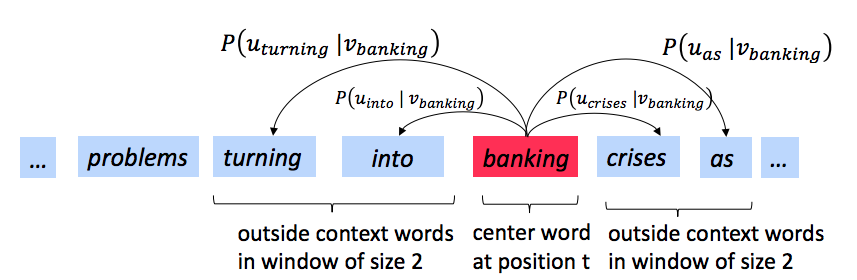
\includegraphics[width=0.6\textwidth]{word2vec.png}
    \caption{The word2vec skip-gram prediction model with window size 2}
    \label{fig:word2vec}
\end{figure}

Skip-gram {\tt word2vec} aims to learn the probability distribution $P(O|C)$. 
Specifically, given a specific word $o$ and a specific word $c$, we want to predict $P(O=o|C=c)$: the probability that word $o$ is an `outside' word for $c$ (i.e., that it falls within the contextual window of $c$).
We model this probability by taking the softmax function over a series of vector dot-products: % I added the word "softmax" here because I bet a lot of students will have forgotten what softmax is and why the loss fn is called naive softmax. but if this is too wordy we can just take it out

\begin{equation}
 P(O=o \mid C=c) = \frac{\exp(\bu_{o}^\top \bv_c)}{\sum_{w \in \text{Vocab}} \exp(\bu_{w}^\top \bv_c)}
 \label{word2vec_condprob}
\end{equation}

For each word, we learn vectors $u$ and $v$, where $\bu_o$ is the `outside' vector representing outside word $o$, and $\bv_c$ is the `center' vector representing center word $c$. 
We store these parameters in two matrices, $\bU$ and $\bV$.
The columns of $\bU$ are all the `outside' vectors $\bu_{w}$;
the columns of $\bV$ are all of the `center' vectors $\bv_{w}$. 
Both $\bU$ and $\bV$ contain a vector for every $w \in \text{Vocabulary}$.\footnote{Assume that every word in our vocabulary is matched to an integer number $k$. Bolded lowercase letters represent vectors. $\bu_{k}$ is both the $k^{th}$ column of $\bU$ and the `outside' word vector for the word indexed by $k$. $\bv_k$ is both the $k^{th}$ column of $\bV$ and the `center' word vector for the word indexed by $k$. \textbf{In order to simplify notation we shall interchangeably use $k$ to refer to word $k$ and the index of word $k$.}}\newline

%We can think of the probability distribution $P(O|C)$ as a prediction function that we can approximate via supervised learning. For any training example, we will have a single $o$ and $c$. We will then compute a value $P(O=o|C=c)$ and report the loss. 
Recall from lectures that, for a single pair of words $c$ and $o$, the loss is given by:

\begin{equation} 
\bJ_{\text{naive-softmax}}(\bv_c, o, \bU) = -\log P(O=o| C=c).
\label{naive-softmax}
\end{equation}

We can view this loss as the cross-entropy\footnote{The \textbf{cross-entropy loss} between the true (discrete) probability distribution $p$ and another distribution $q$ is $-\sum_i p_i \log(q_i)$.} between the true distribution $\by$ and the predicted distribution $\hat{\by}$, for a particular center word c and a particular outside word o. 
Here, both $\by$ and $\hat{\by}$ are vectors with length equal to the number of words in the vocabulary.
Furthermore, the $k^{th}$ entry in these vectors indicates the conditional probability of the $k^{th}$ word being an `outside word' for the given $c$. 
The true empirical distribution $\by$ is a one-hot vector with a 1 for the true outside word $o$, and 0 everywhere else, for this particular example of center word c and outside word o.\footnote{Note that the true conditional probability distribution of context words for the entire training dataset would not be one-hot.}
The predicted distribution $\hat{\by}$ is the probability distribution $P(O|C=c)$ given by our model in equation (\ref{word2vec_condprob}). \newline

\textbf{Note:} Throughout this homework, when computing derivatives, please use the method reviewed during the lecture (i.e. no Taylor Series Approximations).

\clearpage
\begin{parts}
\part[2]
Prove that the naive-softmax loss (Equation \ref{naive-softmax}) is the same as the cross-entropy loss between $\by$  and $\hat{\by}$, i.e. (note that $\by$ 
 (true distribution), $\hat{\by}$ (predicted distribution) are vectors and $\hat{\by}_o$ is a scalar):

\begin{equation} 
-\sum_{w \in \text{Vocab}} \by_w \log(\hat{\by}_w) = - \log (\hat{\by}_o).
\end{equation}

Your answer should be one line. You may describe your answer in words.
\ifans{
\begin{equation} 
\by_w =  
\left\{
    \begin {aligned}
         & 1 \quad & w = o \\
         & 0 \quad & w \neq o                  
    \end{aligned}
\right.
\Rightarrow 
-\sum_{w \in \text{Vocab}} \by_w \log(\hat{\by}_w) = - \log (\hat{\by}_o).
\end{equation}
}
% Question 1-B
\part[6]
\begin{enumerate}[label=\roman*.]
    \item 
    Compute the partial derivative of $\bJ_{\text{naive-softmax}}(\bv_c, o, \bU)$ with respect to $\bv_c$. \emph{Please write your answer in terms of $\by$, $\hat{\by}$, $\bU$, and show your work to receive full credit}.
    \begin{itemize} 
        \item \textbf{Note}: Your final answers for the partial derivative should follow the shape convention: the partial derivative of any function $f(x)$ with respect to $x$ should have the \textbf{same shape} as $x$.\footnote{This allows us to efficiently minimize a function using gradient descent without worrying about reshaping or dimension mismatching. While following the shape convention, we're guaranteed that $\theta:= \theta - \alpha\frac{\partial J(\theta)}{\partial \theta}$ is a well-defined update rule.}
        \item Please provide your answers for the partial derivative in vectorized form. For example, when we ask you to write your answers in terms of $\by$, $\hat{\by}$, and $\bU$, you may not refer to specific elements of these terms in your final answer (such as $\by_1$, $\by_2$, $\dots$). 
    \end{itemize}
    \item
    When is the gradient you computed equal to zero? \\
    \textbf{Hint:} You may wish to review and use some introductory linear algebra concepts.
    \item
    The gradient you found is the difference between the two terms. Provide an interpretation of how each of these terms improves the word vector when this gradient is subtracted from the word vector $v_c$.

\end{enumerate}

\ifans{
\begin{enumerate}[label=\roman*.]
    \item 
    \begin{gather*} 
    \bJ_{\text{naive-softmax}}(\bv_c, o, \bU) = 
    - \log (\hat{\by}_o) = -\log P(O=o| C=c) = -\log ( \frac{\exp(\bu_{o}^\top \bv_c)}{\sum_{w \in \text{Vocab}} \exp(\bu_{w}^\top \bv_c)}) \\
    \nabla_{\bv_c} \bJ_{\text{naive-softmax}}(\bv_c, o, \bU) = 
     \frac{\partial}{\bv_c} (-\log \frac{\exp(\bu_{o}^\top \bv_c)}{\sum_{w \in \text{Vocab}} \exp(\bu_{w}^\top \bv_c)})  = \\
    = -\frac{1}{\hat{\by}_o}  (\frac{ \frac{\partial}{\bv_c} \exp(\bu_{o}^\top \bv_c)}{\sum_{w \in \text{Vocab}} \exp(\bu_{w}^\top \bv_c)} - \frac{\exp(\bu_{o}^\top \bv_c) (\frac{\partial}{\bv_c}\sum_{w \in \text{Vocab}} \exp(\bu_{w}^\top \bv_c))}{(\sum_{w \in \text{Vocab}} \exp(\bu_{w}^\top \bv_c))^2}) = \\ 
    = -\frac{1}{\hat{\by}_o} (\bu_o   \hat{\by}_o - \hat{\by}_o \sum_{w \in \text{Vocab}} \bu_w P(O=w| C=c) = -\bu_o  + \sum_{w \in \text{Vocab}} \bu_w P(O=w| C=c) \\ \\
    \nabla_{\bv_c} \bJ_{\text{naive-softmax}}(\bv_c, o, \bU) = \bu_o  - \sum_{w \in \text{Vocab}} \bu_w P(O=w| C=c) = U^T(\hat{\by} - \by )
    \end{gather*}

    \item 
    The gradient is zero when the predicted output is equal to the expected outpute, i.e. when the calculated mean embedding of all the $\bu_w$ (weighted by their probabilty of ocurrence) is equal to the actual $\bu_o$ observed.

    \item 
    \begin{equation*}
        \bv_c \gets \bv_c - \alpha \bu_o + \alpha \sum_{w \in \text{Vocab}} \bu_w P(O=w| C=c)
    \end{equation*}
    This equation moves the embedding $\bv_c$ in the opposite direction of $\bu_o$ (the embedding of the observed word) and in the direction of the mean embedding, averaged by the probability of ocurrence.
\end{enumerate}
}

% Question 1-C
\part[1]
In many downstream applications using word embeddings, L2 normalized vectors (e.g. $\mathbf{u}/||\mathbf{u}||_2$ where $||\mathbf{u}||_2 = \sqrt{\sum_i u_i^2}$) are used instead of their raw forms (e.g. $\mathbf{u}$). Let’s consider a hypothetical downstream task of binary classification of phrases as being positive or negative, where you decide the sign based on the sum of individual embeddings of the words. When would L2 normalization take away useful information for the downstream task? When would it not?

\ifans{
\begin{gather*}
\bu_x = \alpha \bu_y \Rightarrow L_2(\bu_x) = \frac{\bu_x}{||\bu_x||_2} , L_2(\bu_y)=\frac{\alpha \bu_x}{||\alpha\bu_x||_2} = \frac{\bu_x}{||\bu_x||_2} = L_2(\bu_x)
\end{gather*}
Suppose we have a sentence with both negative (e.g. bad) and positive words (e.g best). In this case best may be $\alpha \bu_x$ where $\bu_x$ could be the word good. In such sentence, summing the bad embedding with the best embedding may classify the sentence as positive. If we apply L2 normalization to the sentence, we will end up summing the embeddings of bad and good that may classify now the sentence as negative. Instead, if we consider the relative positions of the embeddings (not the magnitudes) to make the classification, the L2 normalization will not affect the results.
}

\textbf{Hint:} Consider the case where $\mathbf{u}_x = \alpha\mathbf{u}_y$ for some words $x \neq y$ and some scalar $\alpha$. When $\alpha$ is positive, what will be the value of normalized  $\mathbf{u}_x$ and normalized $\mathbf{u}_y$? How might $\mathbf{u}_x$ and $\mathbf{u}_y$ be related for such a normalization to affect or not affect the resulting classification?


% Question 1-D
\part[5] 
Compute the partial derivatives of $\bJ_{\text{naive-softmax}}(\bv_c, o, \bU)$ with respect to each of the `outside' word vectors, $\bu_w$'s. There will be two cases: when $w=o$, the true `outside' word vector, and $w \neq o$, for all other words. Please write your answer in terms of $\by$, $\hat{\by}$, and $\bv_c$. In this subpart, you may use specific elements within these terms as well (such as $\by_1$, $\by_2$, $\dots$). Note that $\bu_w$ is a vector while $\by_1, \by_2, \dots$ are scalars. Show your work to receive full credit.

\ifans{
\begin{gather*} 
w = o \Rightarrow \nabla_{\bu_o} \bJ_{\text{naive-softmax}}(\bv_c, o, \bU) = 
 \frac{\partial}{\bu_o} (-\log \frac{\exp(\bu_{o}^\top \bv_c)}{\sum_{w \in \text{Vocab}} \exp(\bu_{w}^\top \bv_c)})  = \\
= -\frac{1}{\hat{\by}_o}  (\frac{ \frac{\partial}{\bu_o} \exp(\bu_{o}^\top \bv_c)}{\sum_{w \in \text{Vocab}} \exp(\bu_{w}^\top \bv_c)} - \frac{\exp(\bu_{o}^\top \bv_c) (\frac{\partial}{\bu_o}\sum_{w \in \text{Vocab}} \exp(\bu_{w}^\top \bv_c))}{(\sum_{w \in \text{Vocab}} \exp(\bu_{w}^\top \bv_c))^2}) = \\ 
= -\frac{1}{\hat{\by}_o} (\bv_c \hat{\by}_o - \hat{\by}_o \bv_c \hat{\by}_o) = -\bv_c + \bv_c * \hat{\by}_o
\end{gather*}
\begin{gather*} 
w \neq o \Rightarrow \nabla_{\bu_w} \bJ_{\text{naive-softmax}}(\bv_c, o, \bU) = 
 \frac{\partial}{\bu_w} (-\log \frac{\exp(\bu_{o}^\top \bv_c)}{\sum_{w \in \text{Vocab}} \exp(\bu_{w}^\top \bv_c)})  = \\
= -\frac{1}{\hat{\by}_o}  ( 0 - \frac{\exp(\bu_{o}^\top \bv_c) (\frac{\partial}{\bu_w}\sum_{w \in \text{Vocab}} \exp(\bu_{w}^\top \bv_c))}{(\sum_{w \in \text{Vocab}} \exp(\bu_{w}^\top \bv_c))^2}) = \\ 
= -\frac{1}{\hat{\by}_o} (0 - \hat{\by}_o \sum_{w \in \text{Vocab}} \bv_c P(O=w| C=c) =   \sum_{w \in \text{Vocab}} \bv_c P(O=w| C=c)
\end{gather*}
\begin{gather*} 
\nabla_{\bu_w} \bJ_{\text{naive-softmax}}(\bv_c, o, \bU) = \bv_c( \hat{\by} - \by)
\end{gather*}
}

% Question 1-E
\part[1]
Write down the partial derivative of $\bJ_{\text{naive-softmax}}(\bv_c, o, \bU)$ with respect to $\bU$. Please break down your answer in terms of the column vectors $\frac{\partial \bJ(\bv_c, o, \bU)}{\partial \bu_1}$, $\frac{\partial \bJ(\bv_c, o, \bU)}{\partial \bu_2}$, $\cdots$, $\frac{\partial \bJ(\bv_c, o, \bU)}{\partial \bu_{|\text{Vocab}|}}$. No derivations are necessary, just an answer in the form of a matrix.

\ifans{
\begin{equation*}
     \nabla_{U} \bJ_{\text{naive-softmax}}(\bv_c, o, \bU) = 
     \begin{bmatrix}
     \bv_c \hat{\by_1} \\
     \bv_c \hat{\by_2} \\
     \vdots \\
     \bv_c(\hat{\by_o}-1) \\
     \vdots \\
     \bv_c \hat{y_{|vocab|}} \\
     \end{bmatrix}
\end{equation*}
}

\end{parts}
    \newpage
    \graphicspath{ {images/} }

\titledquestion{Analyzing NMT Systems}[25]

\begin{parts}

    \part[3] Look at the {\monofam{src.vocab}} file for some examples of phrases and words in the source language vocabulary. When encoding an input Mandarin Chinese sequence into ``pieces'' in the vocabulary, the tokenizer maps the sequence to a series of vocabulary items, each consisting of one or more characters (thanks to the {\monofam{sentencepiece}} tokenizer, we can perform this segmentation even when the original text has no white space). Given this information, how could adding a 1D Convolutional layer after the embedding layer and before passing the embeddings into the bidirectional encoder help our NMT system? \textbf{Hint:} each Mandarin Chinese character is either an entire word or a morpheme in a word. Look up the meanings of 电, 脑, and 电脑 separately for an example. The characters 电 (electricity) and  脑 (brain) when combined into the phrase 电脑 mean computer.




    \part[8] Here we present a series of errors we found in the outputs of our NMT model (which is the same as the one you just trained). For each example of a reference (i.e., `gold') English translation, and NMT (i.e., `model') English translation, please:
    
    \begin{enumerate}
        \item Identify the error in the NMT translation.
        \item Provide possible reason(s) why the model may have made the error (either due to a specific linguistic construct or a specific model limitation).
        \item Describe one possible way we might alter the NMT system to fix the observed error. There are more than one possible fixes for an error. For example, it could be tweaking the size of the hidden layers or changing the attention mechanism.
    \end{enumerate}
    
    Below are the translations that you should analyze as described above. Only analyze the underlined error in each sentence. Rest assured that you don't need to know Mandarin to answer these questions. You just need to know English! If, however, you would like some additional color on the source sentences, feel free to use a resource like \url{https://www.archchinese.com/chinese_english_dictionary.html} to look up words. Feel free to search the training data file to have a better sense of how often certain characters occur.

    \begin{subparts}
        \subpart[2]
        \textbf{Source Sentence:} 贼人其后被警方拘捕及被判处盗窃罪名成立。 \newline
        \textbf{Reference Translation:} \textit{\underline{the culprits were} subsequently arrested and convicted.}\newline
        \textbf{NMT Translation:} \textit{\underline{the culprit was} subsequently arrested and sentenced to theft.}
        
        

        \subpart[2]
        \textbf{Source Sentence}: 几乎已经没有地方容纳这些人,资源已经用尽。\newline
        \textbf{Reference Translation}: \textit{there is almost no space to accommodate these people, and resources have run out.   }\newline
        \textbf{NMT Translation}: \textit{the resources have been exhausted and \underline{resources have been exhausted}.}
        
        

        \subpart[2]
        \textbf{Source Sentence}: 当局已经宣布今天是国殇日。 \newline
        \textbf{Reference Translation}: \textit{authorities have announced \underline{a national mourning today.}}\newline
        \textbf{NMT Translation}: \textit{the administration has announced \underline{today's day.}}
        
        
        
        \subpart[2] 
        \textbf{Source Sentence\footnote{This is a Cantonese sentence! The data used in this assignment comes from GALE Phase 3, which is a compilation of news written in simplified Chinese from various sources scraped from the internet along with their translations. For more details, see \url{https://catalog.ldc.upenn.edu/LDC2017T02}. }:} 俗语有云:``唔做唔错"。\newline
        \textbf{Reference Translation:} \textit{\underline{`` act not, err not "}, so a saying goes.}\newline
        \textbf{NMT Translation:} \textit{as the saying goes, \underline{`` it's not wrong. "}}
        
        
    \end{subparts}


    \part[14] BLEU score is the most commonly used automatic evaluation metric for NMT systems. It is usually calculated across the entire test set, but here we will consider BLEU defined for a single example.\footnote{This definition of sentence-level BLEU score matches the \texttt{sentence\_bleu()} function in the \texttt{nltk} Python package. Note that the NLTK function is sensitive to capitalization. In this question, all text is lowercased, so capitalization is irrelevant. \\ \url{http://www.nltk.org/api/nltk.translate.html\#nltk.translate.bleu_score.sentence_bleu}
    } 
    Suppose we have a source sentence $\bs$, a set of $k$ reference translations $\br_1,\dots,\br_k$, and a candidate translation $\bc$. To compute the BLEU score of $\bc$, we first compute the \textit{modified $n$-gram precision} $p_n$ of $\bc$, for each of $n=1,2,3,4$, where $n$ is the $n$ in \href{https://en.wikipedia.org/wiki/N-gram}{n-gram}:
    \begin{align}
        p_n = \frac{ \displaystyle \sum_{\text{ngram} \in \bc} \min \bigg( \max_{i=1,\dots,k} \text{Count}_{\br_i}(\text{ngram}), \enspace \text{Count}_{\bc}(\text{ngram}) \bigg) }{\displaystyle \sum_{\text{ngram}\in \bc} \text{Count}_{\bc}(\text{ngram})}
    \end{align}
     Here, for each of the $n$-grams that appear in the candidate translation $\bc$, we count the maximum number of times it appears in any one reference translation, capped by the number of times it appears in $\bc$ (this is the numerator). We divide this by the number of $n$-grams in $\bc$ (denominator). \newline 

    Next, we compute the \textit{brevity penalty} BP. Let $len(c)$ be the length of $\bc$ and let $len(r)$ be the length of the reference translation that is closest to $len(c)$ (in the case of two equally-close reference translation lengths, choose $len(r)$ as the shorter one). 
    \begin{align}
        BP = 
        \begin{cases}
            1 & \text{if } len(c) \ge len(r) \\
            \exp \big( 1 - \frac{len(r)}{len(c)} \big) & \text{otherwise}
        \end{cases}
    \end{align}
    Lastly, the BLEU score for candidate $\bc$ with respect to $\br_1,\dots,\br_k$ is:
    \begin{align}
        BLEU = BP \times \exp \Big( \sum_{n=1}^4 \lambda_n \log p_n \Big)
    \end{align}
    where $\lambda_1,\lambda_2,\lambda_3,\lambda_4$ are weights that sum to 1. The $\log$ here is natural log.
    \newline
    \begin{subparts}
        \subpart[5] Please consider this example: \newline
        Source Sentence $\bs$: \textbf{需要有充足和可预测的资源。} 
        \newline
        Reference Translation $\br_1$: \textit{resources have to be sufficient and they have to be predictable}
        \newline
        Reference Translation $\br_2$: \textit{adequate and predictable resources are required}
        
        NMT Translation $\bc_1$: there is a need for adequate and predictable resources
        
        NMT Translation $\bc_2$: resources be sufficient and predictable to
        
        Please compute the BLEU scores for $\bc_1$ and $\bc_2$. Let $\lambda_i=0.5$ for $i\in\{1,2\}$ and $\lambda_i=0$ for $i\in\{3,4\}$ (\textbf{this means we ignore 3-grams and 4-grams}, i.e., don't compute $p_3$ or $p_4$). When computing BLEU scores, show your work (i.e., show your computed values for $p_1$, $p_2$, $len(c)$, $len(r)$ and $BP$). Note that the BLEU scores can be expressed between 0 and 1 or between 0 and 100. The code is using the 0 to 100 scale while in this question we are using the \textbf{0 to 1} scale. Please round your responses to 3 decimal places. 
        \newline
        
        Which of the two NMT translations is considered the better translation according to the BLEU Score? Do you agree that it is the better translation?
        
        
        
        \subpart[5] Our hard drive was corrupted and we lost Reference Translation $\br_1$. Please recompute BLEU scores for $\bc_1$ and $\bc_2$, this time with respect to $\br_2$ only. Which of the two NMT translations now receives the higher BLEU score? Do you agree that it is the better translation?
        
        
        
        \subpart[2] Due to data availability, NMT systems are often evaluated with respect to only a single reference translation. Please explain (in a few sentences) why this may be problematic. In your explanation, discuss how the BLEU score metric assesses the quality of NMT translations when there are multiple reference transitions versus a single reference translation.
        
        
        
        \subpart[2] List two advantages and two disadvantages of BLEU, compared to human evaluation, as an evaluation metric for Machine Translation. 
        
        
        
    \end{subparts}


    \part[4] \emph{Beam search} is often employed to improve the quality of machine translation systems. While you were training the model, beam search results for the same example sentence at different iterations were also recorded in TensorBoard, and accessible in the \emph{TEXT} tab (Fig \ref{fig:beam-search-diagnostics-tensorboard}).

    The recorded diagnostic information includes json documents with the following fields: \texttt{example\_source} (the source sentence tokens), \texttt{example\_target} (the ground truth target sentence tokens), and \texttt{hypotheses} (10 hypotheses corresponding to the search result with beam size 10). Note that a predicted translation is often called \emph{hypothesis} in the neural machine translation jargon.

    \begin{subparts}
        \subpart[2] Did the translation quality improve over the training iterations for the model? Give three examples of translations of the example sentence at iterations 200, 3000, and the last iteration to illustrate your answer. For each iteration, pick the first beam search hypothesis as an example:
        
        
        
        
        \subpart[2] How do various hypotheses resulting from beam search qualitatively compare? Give three other examples of hypotheses proposed by beam search at the last iteration to illustrate your answer.
        
        
    \end{subparts}



    \begin{figure}
        \centering
        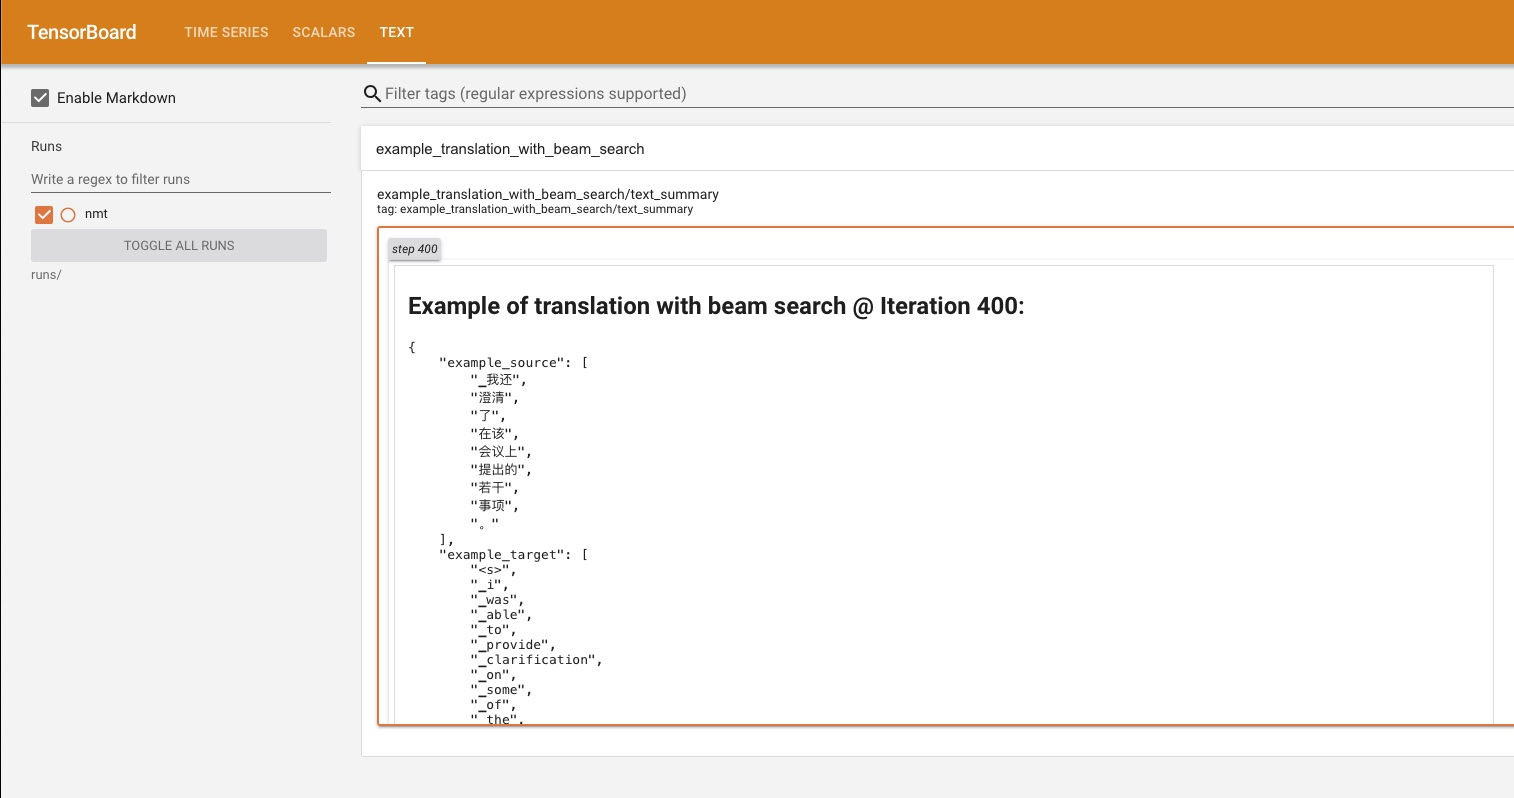
\includegraphics[width=0.7\textwidth]{images/example_translation_beam.jpg}
        \caption{Translation with beam search results for an example sentence are recorded in tensorboard for various iterations. The same data is available in the \texttt{outputs/beam\_search\_diagnostics/} folder in your working directory.}
        \label{fig:beam-search-diagnostics-tensorboard}
    \end{figure}
    

\end{parts}

    \newpage
    \titledquestion{Neural Transition-Based Dependency Parsing}[54]

In this section, you'll be implementing a neural-network based dependency parser with the goal of maximizing performance on the UAS (Unlabeled Attachment Score) metric.\newline

Before you begin, please follow the README to install all the needed dependencies for the assignment. We will be using PyTorch 2.1.2 from \url{https://pytorch.org/get-started/locally/} with the \texttt{CUDA} option set to \texttt{None}, and the tqdm package -- which produces progress bar visualizations throughout your training process. The official PyTorch website is a great resource that includes tutorials for understanding PyTorch's Tensor library and neural networks. \newline

A dependency parser analyzes the grammatical structure of a sentence, establishing relationships between \textit{head} words, and words which modify those heads. There are multiple types of dependency parsers, including transition-based parsers, graph-based parsers, and feature-based parsers. Your implementation will be a {\it transition-based} parser, which incrementally builds up a parse one step at a time. At every step it maintains a \textit{partial parse}, which is represented as follows:
\begin{itemize}
\item A {\it stack} of words that are currently being processed.
\item A {\it buffer} of words yet to be processed.
\item A list of {\it dependencies} predicted by the parser.
\end{itemize}
Initially, the stack only contains ROOT, the dependencies list is empty, and the buffer contains all words of the sentence in order. At each step, the parser applies a {\it transition} to the partial parse until its buffer is empty and the stack size is 1. The following transitions can be applied:
\begin{itemize}
\item \texttt{SHIFT}: removes the first word from the buffer and pushes it onto the stack.
\item \texttt{LEFT-ARC}: marks the second (second most recently added) item on the stack as a dependent of the first item and removes the second item from the stack, adding a \textit{first\_word} $\rightarrow$ \textit{second\_word} dependency to the dependency list.
\item \texttt{RIGHT-ARC}: marks the first (most recently added) item on the stack as a dependent of the second item and removes the first item from the stack, adding a \textit{second\_word} $\rightarrow$ \textit{first\_word} dependency to the dependency list.
\end{itemize}
On each step, your parser will decide among the three transitions using a neural network classifier.

\begin{parts}
    
    \part[4] \textcolor{black}{Go through the sequence of transitions needed for parsing the sentence {\it ``I presented my findings at the NLP conference''}. The dependency tree for the sentence is shown below. At each step, give the configuration of the stack and buffer, as well as what transition was applied this step and what new dependency was added (if any). The first three steps are provided below as an example.} \\

    %\begin{center}
    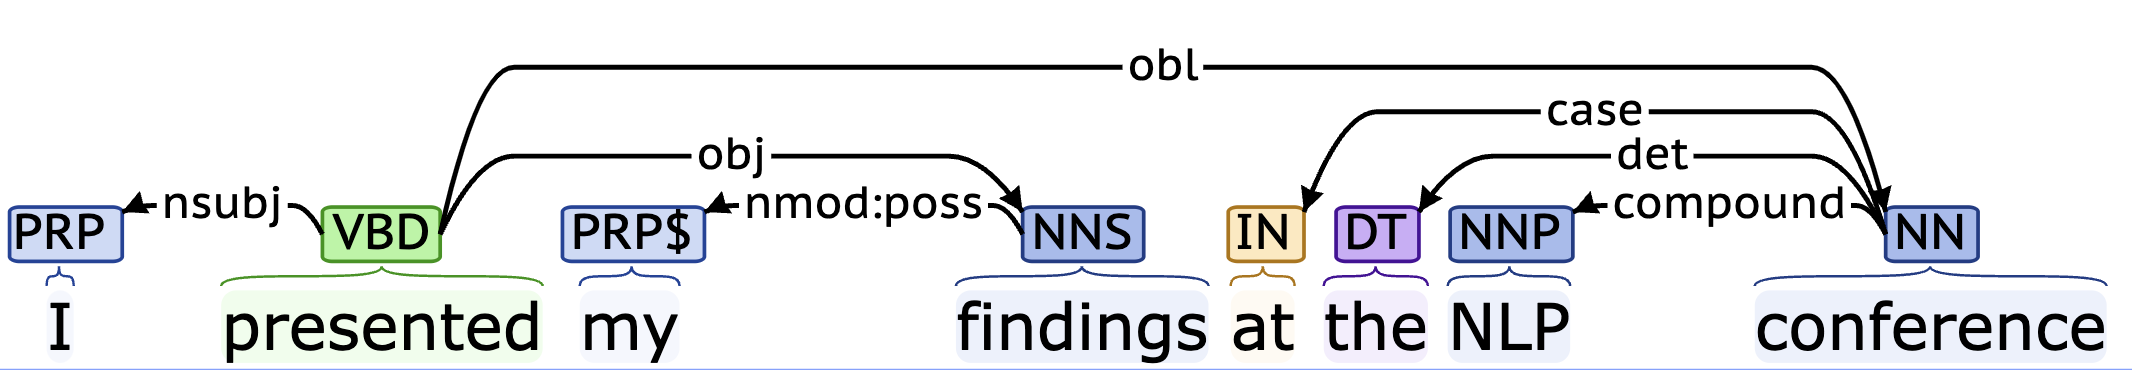
\includegraphics[width=0.8\textwidth]{example.png} \\
    %\end{center}

    \begin{adjustwidth}{-2cm}{}
    \begin{tabular}{ l | l | l | l}
    Stack & Buffer & New dependency & Transition \\ \hline
    [ROOT] & [I, presented, my, findings, at, the, NLP, conference] &  & Initial Configuration \\
    $[$ROOT, I] & [presented, my, findings, at, the, NLP, conference] &  &  \texttt{SHIFT}  \\
    $[$ROOT, I, presented] & [my, findings, at, the, NLP, conference] &  &  \texttt{SHIFT}  \\
    $[$ROOT, presented] & [my, findings, at, the, NLP, conference] & presented$\to$I &  \texttt{LEFT-ARC}  \\
    \end{tabular}\newline
    \end{adjustwidth}

\ifans{
\newline
\resizebox{\textwidth}{!}{%
    \begin{tabular}{ l | l | l | l}
    Stack & Buffer & New dependency & Transition \\ \hline
    [ROOT] & [I, presented, my, findings, at, the, NLP, conference] &  & Initial Configuration \\
    $[$ROOT, I] & [presented, my, findings, at, the, NLP, conference] &  &  \texttt{SHIFT}  \\
    $[$ROOT, I, presented] & [my, findings, at, the, NLP, conference] &  &  \texttt{SHIFT}  \\
    $[$ROOT, presented] & [my, findings, at, the, NLP, conference] & presented$\to$I &  \texttt{LEFT-ARC}  \\
    $[$ROOT, presented, my] & [findings, at, the, NLP, conference] &  &  \texttt{SHIFT} \\
    $[$ROOT, presented, my, findings] & [at, the, NLP, conference] &  &  \texttt{SHIFT} \\
    $[$ROOT, presented, findings] & [at, the, NLP, conference] & findings$\to$my  &  \texttt{LEFT-ARC} \\
    $[$ROOT, presented] & [at, the, NLP, conference] & presented$\to$findings  &  \texttt{RIGHT-ARC} \\
    $[$ROOT, presented, at] & [the, NLP, conference] &  &  \texttt{SHIFT} \\
    $[$ROOT, presented, at, the] & [NLP, conference] &  &  \texttt{SHIFT} \\
    $[$ROOT, presented, at, the, NLP] & [conference] &  &  \texttt{SHIFT} \\
    $[$ROOT, presented, at, the, NLP, conference] & [] &  &  \texttt{SHIFT} \\
    $[$ROOT, presented, at, the, conference] & [] & conference$\to$NLP &  \texttt{LEFT-ARC} \\
    $[$ROOT, presented, at, conference] & [] & conference$\to$the &  \texttt{LEFT-ARC} \\
    $[$ROOT, presented, conference] & [] & conference$\to$at &  \texttt{LEFT-ARC} \\
    $[$ROOT, presented] & [] & presented$\to$conference &  \texttt{RIGHT-ARC} \\
    $[$ROOT] & [] & ROOT$\to$presented &  \texttt{LEFT-ARC} \\
    \end{tabular}}
}
    
    \part[2] A sentence containing $n$ words will be parsed in how many steps (in terms of $n$)? Briefly explain in 1--2 sentences why.

\ifans{
We will need $2*n$ steps. For each word we need one operation to move the word from the buffer to the stack and another operation to create the relationship that removes the word from the stack.
}
    
    \part[6] Implement the \texttt{\_\_init\_\_} and \texttt{parse\_step} functions in the \texttt{PartialParse} class in \texttt{parser\_transitions.py}. This implements the transition mechanics your parser will use. You can run basic (non-exhaustive) tests by running \texttt{python parser\_transitions.py part\_c}.

    \part[8] Our network will predict which transition should be applied next to a partial parse. We could use it to parse a single sentence by applying predicted transitions until the parse is complete. However, neural networks run much more efficiently when making predictions about \textit{batches} of data at a time (i.e., predicting the next transition for any different partial parses simultaneously). We can parse sentences in minibatches with the following algorithm. \newline

    \alglanguage{pseudocode}
    \begin{algorithm*}[h]
    \caption{Minibatch Dependency Parsing}
    \begin{algorithmic}
    	\State \textbf{Input:} \texttt{sentences}, a list of sentences to be parsed and \texttt{model}, our model that makes parse decisions
    	%\State
    	%\State Initialize \texttt{partial\_parses} $\to$ []
    	%\For{\textbf{each} sentence \texttt{s} in \texttt{sentences}}
    	%	\State Add a partial parse to \texttt{partial\_parses} with \texttt{stack} = [ROOT], \texttt{buffer} = \texttt{s}, \texttt{dependencies} = []
    	%\EndFor
    	\State
    	\State Initialize \texttt{partial\_parses} as a list of PartialParses, one for each sentence in \texttt{sentences}
    	\State Initialize \texttt{unfinished\_parses} as a shallow copy of \texttt{partial\_parses}
    	%\State
    	\While{\texttt{unfinished\_parses} is not empty}

    		\State Take the first \texttt{batch\_size} parses in \texttt{unfinished\_parses} as a minibatch
    		\State Use the \texttt{model} to predict the next transition for each partial parse in the minibatch
    		\State Perform a parse step on each partial parse in the minibatch with its predicted transition
    		\State Remove the completed (empty buffer and stack of size 1) parses from \texttt{unfinished\_parses}
    	\EndWhile
    	\State
    	\State \textbf{Return:} The \texttt{dependencies} for each (now completed) parse in \texttt{partial\_parses}.
    \end{algorithmic}
    \end{algorithm*}
    
    Implement this algorithm in the \texttt{minibatch\_parse} function in \texttt{parser\_transitions.py}. You can run basic (non-exhaustive) tests by running \texttt{python parser\_transitions.py part\_d}.

    {\it Note: You will need \texttt{minibatch\_parse} to be correctly implemented to evaluate the model you will build in part (e). However, you do not need it to train the model, so you should be able to complete most of part (e) even if \texttt{minibatch\_parse} is not implemented yet.} \newline
    
    \part[20] We are now going to train a neural network to predict, given the state of the stack, buffer, and dependencies, which transition should be applied next.
    
    First, the model extracts a feature vector representing the current state. We will be using the feature set presented in the original neural dependency parsing paper: {\it A Fast and Accurate Dependency Parser using Neural Networks}.\footnote{Chen and Manning, 2014, \url{https://nlp.stanford.edu/pubs/emnlp2014-depparser.pdf}} The function extracting these features has been implemented for you in \texttt{utils/parser\_utils.py}. This feature vector consists of a list of tokens (e.g., the last word in the stack, first word in the buffer, dependent of the second-to-last word in the stack if there is one, etc.). They can be represented as a list of integers $\bw = [w_1, w_2, \dots, w_m]$ where $m$ is the number of features and each $0 \leq w_i < |V|$ is the index of a token in the vocabulary ($|V|$ is the vocabulary size). Then our network looks up an embedding for each word and concatenates them into a single input vector:
    \alns{
    	\bx = [\bE_{w_1}, ..., \bE_{w_m }] \in \mathbb{R}^{dm}
    }
    where $\bE \in \mathbb{R}^{|V| \times d}$ is an embedding matrix with each row $\bE_w$ as the vector for a particular word $w$ with dimension d. We then compute our prediction as:
    \alns{
    	\bh &= \relu(\bx \bW   + \bb_1) \\
    	\bl &= \bh \bU + \bb_2 \\
    	\byt &= \smx(l) \\
    }
    where \bh \space is referred to as the hidden layer, \bl \space is referred to as the logits, $\byt$ \space is referred to as the predictions, and $\relu(z) = \max(z, 0)$). We will train the model to minimize cross-entropy loss:
    \alns{
    	J(\theta) &= CE(\by, \byt) = -\sum \limits_{j = 1}^{3} \by_j \log \byt_j
    } where $\by_j$ denotes the $j$th element of $\by$.
    To compute the loss for the training set, we average this $J(\theta)$ across all training examples.
    
    \begin{enumerate}[label=\roman*.]
    
        \item \textcolor{black}{Compute the derivative of $\bh = \relu(\bx \bW + \bb_1)$ with respect to $\bx$. For simplicity, you only need to show the derivative $\frac{\partial h_i}{\partial x_j}$ for some index $i$ and $j$. You may ignore the case where the derivative is not defined at 0.}
        \item \textcolor{black}{Recall in part 1b, we computed the partial derivative of $\bJ_{\text{naive-softmax}}(\bv_c, o, \bU)$. Likewise, please compute the partial derivative of $J(\theta)$ with respect to the $i$th entry of $\bl$, which is denoted as $\bl_i$. Specifically, compute $\frac{\partial CE(\by, \byt)}{\partial \bl_i}$, assuming that $\bl \in \R^3$, $\byt \in \R^3$, $\by \in \R^3$, and the true label is $c$. \\
        \textbf{Hints}: You may recall from part 1a, $\frac{\partial CE(\by, \byt)}{\partial \bl_i} = \sum_j \frac{\partial CE(\by, \byt)}{\partial \byt_j}\frac{\partial \byt_j}{\partial \bl_i}$, and $\frac{\partial CE(\by, \byt)}{\partial \byt_j}=0$ if $j \neq c$. 
        }
        \item We will use UAS score as our evaluation metric. UAS refers to Unlabeled Attachment Score, which is computed as the ratio between number of correctly predicted dependencies and the number of total dependencies despite of the relations (our model doesn't predict this).\newline
    
   In \texttt{parser\_model.py} you will find skeleton code to implement this simple neural network using PyTorch. Complete the \texttt{\_\_init\_\_}, \texttt{embedding\_lookup} and \texttt{forward} functions to implement the model. Then complete the \texttt{train\_for\_epoch} and \texttt{train} functions within the \texttt{run.py} file.
   
    Finally execute \texttt{python run.py} to train your model and compute predictions
    on test data from Penn Treebank (annotated with Universal Dependencies). 
    
    \textbf{Note:}
    \begin{itemize}
        \item For this assignment, you are asked to implement Linear layer and Embedding layer. Please \textbf{DO NOT} use \textbf{torch.nn.Linear} or  \textbf{torch.nn.Embedding} module in your code, otherwise you will receive deductions for this problem. 
        \item Please follow the naming requirements in our TODO if there are any, e.g. if there are explicit requirements about variable names you have to follow them in order to receive full credits. You are free to declare other variable names if not explicitly required. 
    \end{itemize}
    
    \textbf{Hints:}
    \begin{itemize}
        \item Each of the variables you are asked to declare (\texttt{self.embed\_to\_hidden\_weight}, \newline \texttt{self.embed\_to\_hidden\_bias}, \texttt{self.hidden\_to\_logits\_weight}, \newline \texttt{self.hidden\_to\_logits\_bias}) corresponds to one of the variables above (\bW, $\bb_1$, \bU, $\bb_2$).  
        \item It may help to work backwards in the algorithm (start from $\byt$) and keep track of the matrix/vector sizes.  
        \item Once you have implemented \texttt{embedding\_lookup (e)} or \texttt{forward (f)} you can call \texttt{python parser\_model.py} with flag \texttt{-e} or \texttt{-f} or both to run sanity checks with each function. These sanity checks are fairly basic and passing them doesn't mean your code is bug free.
        \item
            When debugging, you can add a debug flag: \texttt{python run.py -d}. This will cause the code to run over a small subset of the data, so that training the model won't take as long. Make sure to remove the \texttt{-d} flag to run the full model once you are done debugging.

        \item
            When running with debug mode, you should be able to get a loss smaller than 0.2 and a UAS larger than 65 on the dev set (although in rare cases your results may be lower, there is some randomness when training).
        
        \item It should take up to \textbf{15 minutes} to train the model on the entire training dataset, i.e., when debug mode is disabled.
        
        \item When debug mode is disabled, you should be able to get a loss smaller than 0.08 on the train set and an Unlabeled Attachment Score larger than 87 on the dev set. For comparison, the model in the original neural dependency parsing paper gets 92.5 UAS. If you want, you can tweak the hyperparameters for your model (hidden layer size, hyperparameters for Adam, number of epochs, etc.) to improve the performance (but you are not required to do so).
    \end{itemize}
    
    \textbf{Deliverables:}
        \begin{itemize}
            \item Working implementation of the transition mechanics that the neural dependency parser uses in \texttt{parser\_transitions.py}. 
            \item Working implementation of minibatch dependency parsing in \texttt{parser\_transitions.py}. 
            \item Working implementation of the neural dependency parser in \texttt{parser\_model.py}. (We'll look at and run this code for grading).
            \item Working implementation of the functions for training in \texttt{run.py}. (We'll look at and run this code for grading).
            \item \textbf{Report the best UAS your model achieves on the dev set and the UAS it achieves on the test set in your written submission}.
    \end{itemize}
    \end{enumerate}
    
    
\part[12] We'd like to look at example dependency parses and understand where parsers like ours might be wrong. For example, in this sentence:

\begin{center}
 {
 \begin{dependency}
 \begin{deptext}
Moscow  \& sent \& troops \& into  \& Afghanistan \& .     \\
 PROPN \& VERB  \& NOUN  \& ADP \& PROPN \& PUNCT \\
 \end{deptext}
 \depedge{2}{1}{nsubj}
 \depedge{2}{3}{dobj}
 \deproot{2}{root}
 \depedge{3}{5}{nmod}
 \depedge{5}{4}{case}
 \depedge[edge unit distance=2.25ex]{2}{6}{punct}
 \end{dependency}
 }
 \end{center}

the dependency of the phrase \emph{into Afghanistan} is wrong, because the phrase should modify \emph{sent} (as in \textit{sent into Afghanistan}) not \emph{troops} (because \textit{troops into Afghanistan} doesn't make sense, unless there are somehow weirdly some troops that stan Afghanistan). Here is the correct parse:

\begin{center}
 {
 \begin{dependency}
 \begin{deptext}
Moscow  \& sent \& troops \& into  \& Afghanistan \& .     \\
 PROPN \& VERB  \& NOUN  \& ADP \& PROPN \& PUNCT \\
 \end{deptext}
 \depedge{2}{1}{nsubj}
 \depedge{2}{3}{dobj}
 \deproot{2}{root}
 \depedge[edge unit distance=2ex]{2}{5}{nmod}
 \depedge{5}{4}{case}
 \depedge[edge unit distance=2.25ex]{2}{6}{punct}
 \end{dependency}
 }
 \end{center}

More generally, here are four types of parsing error:
\begin{itemize}
    \item \textbf{Prepositional Phrase Attachment Error}: In the example above, the phrase \textit{into Afghanistan} is a prepositional phrase\footnote{For examples of prepositional phrases, see: https://www.grammarly.com/blog/prepositional-phrase/}.
    A Prepositional Phrase Attachment Error is when a prepositional phrase is attached to the wrong head word (in this example, \textit{troops} is the wrong head word and \textit{sent} is the correct head word).
    More examples of prepositional phrases include \textit{with a rock}, \textit{before midnight} and \textit{under the carpet}. 
    \item \textbf{Verb Phrase Attachment Error}: In the sentence \textit{Leaving the store unattended, I went outside to watch the parade}, the phrase \textit{leaving the store unattended} is a verb phrase\footnote{For examples of verb phrases, see: https://examples.yourdictionary.com/verb-phrase-examples.html}. 
    A Verb Phrase Attachment Error is when a verb phrase is attached to the wrong head word (in this example, the correct head word is \textit{went}).
    \item \textbf{Modifier Attachment Error}: In the sentence \textit{I am extremely short}, the adverb \textit{extremely} is a modifier of the adjective \textit{short}. A Modifier Attachment Error is when a modifier is attached to the wrong head word (in this example, the correct head word is \textit{short}).
    \item \textbf{Coordination Attachment Error}: In the sentence \textit{Would you like brown rice or garlic naan?}, the phrases \textit{brown rice} and \textit{garlic naan} are both conjuncts and the word \textit{or} is the coordinating conjunction. The second conjunct (here \textit{garlic naan}) should be attached to the first conjunct (here \textit{brown rice}). A Coordination Attachment Error is when the second conjunct is attached to the wrong head word (in this example, the correct head word is \textit{rice}). Other coordinating conjunctions include \textit{and}, \textit{but} and \textit{so}.
\end{itemize}
In this question are four sentences with dependency parses obtained from a parser. Each sentence has one error type, and there is one example of each of the four types above. 
For each sentence, state the type of error, the incorrect dependency, and the correct dependency. While each sentence should have a unique error type, there may be multiple possible correct dependencies for some of the sentences.
To demonstrate: for the example above, you would write: 
\begin{itemize}
    \item \textbf{Error type}: Prepositional Phrase Attachment Error 
    \item \textbf{Incorrect dependency}: troops $\rightarrow$ Afghanistan 
    \item \textbf{Correct dependency}: sent $\rightarrow$ Afghanistan
\end{itemize}

\textit{\textbf{Note}: 
There are lots of details and conventions for dependency annotation. 
If you want to learn more about them, you can look at the UD website: \url{http://universaldependencies.org}\footnote{But note that in the assignment we are actually using UDv1, see: \url{http://universaldependencies.org/docsv1/}} or the short introductory slides at: \url{http://people.cs.georgetown.edu/nschneid/p/UD-for-English.pdf}.
Note that you \textbf{do not} need to know all these details in order to do this question. In each of these cases, we are asking about the attachment of phrases and it should be sufficient to see if they are modifying the correct head.
In particular, you \textbf{do not} need to look at the labels on the the dependency edges -- it suffices to just look at the edges themselves. }

\medskip

i. \\
\begin{center}
{

\begin{dependency}[] 
 \begin{deptext}
The \& university \& blocked \& the \& acquisition \& , \& citing \& concerns \& about \& the \& risks \& involved \& . \\
DET \& NOUN \& VERB \& DET \& NOUN \& PUNCT \& VERB \& NOUN \& ADP \& DET \& NOUN \& VERB \& PUNCT \\
\end{deptext}
\depedge{2}{1}{det}
\depedge{3}{2}{nsubj}
\deproot[edge unit distance=5ex]{3}{root}
\depedge{5}{4}{det}
\depedge{3}{5}{obj}
\depedge{7}{6}{punct}
\depedge{5}{7}{advcl}
\depedge{7}{8}{obj}
\depedge{11}{9}{case}
\depedge{11}{10}{det}
\depedge{8}{11}{nmod}
\depedge{11}{12}{acl}
\depedge[edge unit distance=1.7ex]{3}{13}{punct}
\end{dependency}
 }
 \end{center}

%%%%%%%%%%%%%%%%%%%%%%%%%%%%%%%

ii. \\
 \begin{center}
 \color{black}
 {\small
 \begin{dependency}
 \begin{deptext}
 Brian \& has \& been \& one \& of  \& the \& most \& crucial \& elements \& to  \& the \& success \& of  \& Mozilla \& software \& .     \\
 PROPN \& AUX \& AUX  \& NUM \& ADP \& DET \& ADV  \& ADJ     \& NOUN     \& ADP \& DET \& NOUN    \& ADP \& PROPN   \& NOUN \& PUNCT \\
 \end{deptext}
 \depedge{4}{1}{nsubj}
 \depedge{4}{2}{aux}
 \depedge{4}{3}{aux}
 \deproot[edge unit distance=5.5ex]{4}{root}
 \depedge{9}{5}{case}
 \depedge{9}{6}{det}
 \depedge{9}{7}{advmod}
 \depedge{9}{8}{amod}
 \depedge{4}{9}{nmod}
 \depedge{12}{10}{case}
 \depedge{12}{11}{det}
 \depedge{9}{12}{nmod}
 \depedge{15}{13}{case}
 \depedge{15}{14}{compound}
 \depedge{12}{15}{nmod}
 \depedge[edge unit distance=1.65ex]{4}{16}{punct}
 \end{dependency}
 }
 \end{center}

%%%%%%%%%%%%%%%%%%%%%%%%%%%%%%%

\medskip

iii. \\
\begin{center}
 {\small

 \begin{dependency}[] 
 \begin{deptext}
Investment \& Canada \& declined \& to \& comment \& on \& the \& reasons \& for \& the \& goverment \& decision \& . \\
NOUN \& PROPN \& VERB \& PART \& VERB \& ADP \& DET \& NOUN \& ADP \& DET \& NOUN \& NOUN \& PUNCT \\
\end{deptext}
\depedge{2}{1}{compound}
\depedge{3}{2}{nsubj}
\deproot[edge unit distance=5.75ex]{3}{root}
\depedge{5}{4}{mark}
\depedge{3}{5}{xcomp}
\depedge{8}{6}{case}
\depedge{8}{7}{det}
\depedge{5}{8}{obl}
\depedge{12}{9}{case}
\depedge{12}{10}{det}
\depedge{12}{11}{compound}
\depedge[edge unit distance=1.5ex]{3}{12}{nmod}
\depedge[edge unit distance=1.7ex]{3}{13}{punct}
\end{dependency}

 }
 \end{center}

iv. \\
 \begin{center}
 {\small
 \begin{dependency}[] 
 \begin{deptext}
People \& benefit \& from \& a \& separate \& move \& that \& affects \& three \& US \& car \& plants \& and \& one \& in \& Quebec \\
NOUN \& VERB \& ADP \& DET \& ADJ \& NOUN \& PRON \& VERB \& NUM \& PROPN \& NOUN \& NOUN \& CCONJ \& NUM \& ADP \& PROPN \\
\end{deptext}
\depedge{2}{1}{nsubj}
\deproot[edge unit distance=3ex]{2}{root}
\depedge{6}{3}{case}
\depedge{6}{4}{det}
\depedge{6}{5}{amod}
\depedge{2}{6}{obl}
\depedge{8}{7}{nsubj}
\depedge{6}{8}{acl:relcl}
\depedge{12}{9}{nummod}
\depedge{12}{10}{compound}
\depedge{12}{11}{compound}
\depedge{8}{12}{obj}
\depedge{14}{13}{cc}
\depedge{8}{14}{conj}
\depedge{16}{15}{case}
\depedge{14}{16}{nmod}
\end{dependency}
 }
 \end{center}

\ifans{
\begin{enumerate}[label=\roman*.]

\item 
\begin{itemize}
    \item \textbf{Error type}: Verb Phrase Attachment Error 
    \item \textbf{Incorrect dependency}: acquisition $\rightarrow$ citing 
    \item \textbf{Correct dependency}: blocked $\rightarrow$ citing \\
\end{itemize}

\item 
\begin{itemize}
    \item \textbf{Error type}: Modifier Attachment Error 
    \item \textbf{Incorrect dependency}: elements $\rightarrow$ most
    \item \textbf{Correct dependency}: crucial $\rightarrow$ most \\
\end{itemize}

\item 
\begin{itemize}
    \item \textbf{Error type}: Prepositional Phrase Attachment Error 
    \item \textbf{Incorrect dependency}: comment $\rightarrow$ reasons
    \item \textbf{Correct dependency}: declined $\rightarrow$ reasons \\
\end{itemize}

\item 
\begin{itemize}
    \item \textbf{Error type}: Coordination Attachment Error 
    \item \textbf{Incorrect dependency}: affects $\rightarrow$ one 
    \item \textbf{Correct dependency}: plants $\rightarrow$ one \\
\end{itemize}
\end{enumerate}
}



\part[2] Recall in part (e), the parser uses features which includes words and their part-of-speech (POS) tags. Explain the benefit of using part-of-speech tags as features in the parser?

\end{parts}

\end{questions}

\Large{\textbf{Submission Instructions}}

\normalsize
You shall submit this assignment on GradeScope as two submissions -- one for ``Assignment 3 [coding]" and another for `Assignment 3 [written]":
\begin{enumerate}
    \item Run the \texttt{collect\_submission.sh} script on the cloud VM to produce your \texttt{assignment3.zip} file. See \emph{How to Download the Gradescope Submission Package from Your Cloud VM} in the GCP How-to Appendix.
    \item Upload your \texttt{assignment3.zip} file to GradeScope to ``Assignment 3 [coding]".
    \item Upload your written solutions to GradeScope to ``Assignment 3 [written]". When you submit your assignment, make sure to tag all the pages for each problem according to Gradescope's submission directions. Points will be deducted if the submission is not correctly tagged.
\end{enumerate}
\end{document}